\documentclass[a4paper,11pt,fleqn,twoside,openright,oldfontcommand]{memoir} 	% Openright aabner kapitler paa hoejresider (openany begge)

%%%% PAKKER %%%%

% ¤¤ Oversaettelse og tegnsaetning ¤¤ %
\usepackage[utf8]{inputenc}					% Input-indkodning af tegnsaet (UTF8)
\usepackage[danish]{babel}					% Dokumentets sprog
\usepackage[T1]{fontenc}					% Output-indkodning af tegnsaet (T1)
\usepackage{ragged2e,anyfontsize}			% Justering af elementer
\usepackage{fixltx2e}						% Retter forskellige fejl i LaTeX-kernen
			
																
% ¤¤ Figurer og tabeller (floats) ¤¤ %
\usepackage{graphicx} 						% Haandtering af eksterne billeder (JPG, PNG, PDF)
\usepackage{multirow}                		% Fletning af raekker og kolonner (\multicolumn og \multirow)
\usepackage{colortbl} 						% Farver i tabeller (fx \columncolor, \rowcolor og \cellcolor)
\usepackage[dvipsnames]{xcolor}				% Definer farver med \definecolor. Se mere: http://en.wikibooks.org/wiki/LaTeX/Colors
\usepackage{flafter}						% Soerger for at floats ikke optraeder i teksten foer deres reference
\let\newfloat\relax 						% Justering mellem float-pakken og memoir
\usepackage{float}							% Muliggoer eksakt placering af floats, f.eks. \begin{figure}[H]
%\usepackage{eso-pic}						% Tilfoej billedekommandoer paa hver side
%\usepackage{wrapfig}						% Indsaettelse af figurer omsvoebt af tekst. \begin{wrapfigure}{Placering}{Stoerrelse}
%\usepackage{multicol}         	        	% Muliggoer tekst i spalter
%\usepackage{rotating}						% Rotation af tekst med \begin{sideways}...\end{sideways}

% ¤¤ Matematik mm. ¤¤
\usepackage{amsmath,amssymb,stmaryrd} 		% Avancerede matematik-udvidelser
\usepackage{mathtools}						% Andre matematik- og tegnudvidelser
\usepackage{textcomp}                 		% Symbol-udvidelser (f.eks. promille-tegn med \textperthousand )
\usepackage{siunitx}						% Flot og konsistent praesentation af tal og enheder med \si{enhed} og \SI{tal}{enhed}
\sisetup{output-decimal-marker = {,}}		% Opsaetning af \SI (DE for komma som decimalseparator) 
\usepackage[version=3]{mhchem} 				% Kemi-pakke til flot og let notation af formler, f.eks. \ce{Fe2O3}
%\usepackage{rsphrase}						% Kemi-pakke til RS-saetninger, f.eks. \rsphrase{R1}

% ¤¤ Referencer og kilder ¤¤ %
\usepackage[danish]{varioref}				% Muliggoer bl.a. krydshenvisninger med sidetal (\vref)
\usepackage[numbers,sort&compress]{natbib}

% ¤¤ Misc. ¤¤ %
\usepackage{listings}						% Placer kildekode i dokumentet med \begin{lstlisting}...\end{lstlisting}
\usepackage{lipsum}							% Dummy text \lipsum[..]
\usepackage[shortlabels]{enumitem}			% Muliggoer enkelt konfiguration af lister
\usepackage{pdfpages}						% Goer det muligt at inkludere pdf-dokumenter med kommandoen \includepdf[pages={x-y}]{fil.pdf}	
\pdfoptionpdfminorversion=6					% Muliggoer inkludering af pdf dokumenter, af version 1.6 og hoejere
\pretolerance=2500 							% Justering af afstand mellem ord (hoejt tal, mindre orddeling og mere luft mellem ord)
\usepackage{geometry}
\usepackage{titlesec}  						%needs recent version of »titlesec«
\usepackage{xcolor}

% Kommentarer og rettelser med \fxnote. Med 'final' i stedet for 'draft' udloeser hver note en error i den faerdige rapport.
\usepackage[footnote,draft,danish,silent,nomargin]{fixme}		


%%%% BRUGERDEFINEREDE INDSTILLINGER %%%%

% ¤¤ Marginer ¤¤ %
\setlrmarginsandblock{3.0cm}{3.0cm}{*}		% \setlrmarginsandblock{Indbinding}{Kant}{Ratio}
\setulmarginsandblock{3.0cm}{3.0cm}{*}		% \setulmarginsandblock{Top}{Bund}{Ratio}
\checkandfixthelayout 						% Oversaetter vaerdier til brug for andre pakker

%	¤¤ Afsnitsformatering ¤¤ %
\setlength{\parindent}{0mm}           		% Stoerrelse af indryk
\setlength{\parskip}{3mm}          			% Afstand mellem afsnit ved brug af double Enter
\linespread{1,1}							% Linie afstand

% ¤¤ Litteraturlisten ¤¤ %
\bibliographystyle{unsrtnat}

% ¤¤ Indholdsfortegnelse ¤¤ %
\setsecnumdepth{subsection}		 			% Dybden af nummerede overkrifter (part/chapter/section/subsection)
\maxsecnumdepth{subsection}					% Dokumentklassens graense for nummereringsdybde
\settocdepth{subsection} 					% Dybden af indholdsfortegnelsen

% ¤¤ Lister ¤¤ %
\setlist{
  topsep=0pt,								% Vertikal afstand mellem tekst og listen
  itemsep=-1ex,								% Vertikal afstand mellem items
} 

% ¤¤ Visuelle referencer ¤¤ %
\usepackage[colorlinks]{hyperref}			% Danner klikbare referencer (hyperlinks) i dokumentet.
\hypersetup{colorlinks = true,				% Opsaetning af farvede hyperlinks (interne links, citeringer og URL)
    linkcolor = black,
    citecolor = black,
    urlcolor = black
}

% ¤¤ Opsaetning af figur- og tabeltekst ¤¤ %
\captionnamefont{\small\bfseries\itshape}	% Opsaetning af tekstdelen ('Figur' eller 'Tabel')
\captiontitlefont{\small}					% Opsaetning af nummerering
\captiondelim{. }							% Seperator mellem nummerering og figurtekst
\hangcaption								% Venstrejusterer flere-liniers figurtekst under hinanden
\captionwidth{\linewidth}					% Bredden af figurteksten
\setlength{\belowcaptionskip}{0pt}			% Afstand under figurteksten
		
% ¤¤ Opsaetning af listings ¤¤ %
\definecolor{commentGreen}{RGB}{34,139,24}
\definecolor{stringPurple}{RGB}{208,76,239}

\lstset{language=Matlab,					% Sprog
	basicstyle=\ttfamily\scriptsize,		% Opsaetning af teksten
	keywords={for,if,while,else,elseif,		% Noegleord at fremhaeve
			  end,break,return,case,
			  switch,function},
	keywordstyle=\color{blue},				% Opsaetning af noegleord
	commentstyle=\color{commentGreen},		% Opsaetning af kommentarer
	stringstyle=\color{stringPurple},		% Opsaetning af strenge
	showstringspaces=false,					% Mellemrum i strenge enten vist eller blanke
	numbers=left, numberstyle=\tiny,		% Linjenumre
	extendedchars=true, 					% Tillader specielle karakterer
	columns=flexible,						% Kolonnejustering
	breaklines, breakatwhitespace=true,		% Bryd lange linjer
}

% ¤¤ Navngivning ¤¤ %
\addto\captionsdanish{
	\renewcommand\appendixname{Bilag}
	\renewcommand\contentsname{Indholdsfortegnelse}	
	\renewcommand\appendixpagename{Bilag}
	\renewcommand\appendixtocname{Bilag}
	\renewcommand\cftchaptername{\chaptername~}				% Skriver "Kapitel" foran kapitlerne i indholdsfortegnelsen
	\renewcommand\cftappendixname{\appendixname~}			% Skriver "Appendiks" foran appendiks i indholdsfortegnelsen
}

% ¤¤ Kapiteludssende ¤¤ %
\definecolor{numbercolor}{gray}{0.7}		% Definerer en farve til brug til kapiteludseende
\newif\ifchapternonum

\makechapterstyle{jenor}{					% Definerer kapiteludseende frem til ...
  \renewcommand\beforechapskip{0pt}
  \renewcommand\printchaptername{}
  \renewcommand\printchapternum{}
  \renewcommand\printchapternonum{\chapternonumtrue}
  \renewcommand\chaptitlefont{\fontfamily{pbk}\fontseries{db}\fontshape{n}\fontsize{25}{35}\selectfont\raggedleft}
  \renewcommand\chapnumfont{\fontfamily{pbk}\fontseries{m}\fontshape{n}\fontsize{1in}{0in}\selectfont\color{numbercolor}}
  \renewcommand\printchaptertitle[1]{%
    \noindent
    \ifchapternonum
    \begin{tabularx}{\textwidth}{X}
    {\let\\\newline\chaptitlefont ##1\par} 
    \end{tabularx}
    \par\vskip-2.5mm\hrule
    \else
    \begin{tabularx}{\textwidth}{Xl}
    {\parbox[b]{\linewidth}{\chaptitlefont ##1}} & \raisebox{-15pt}{\chapnumfont \thechapter}
    \end{tabularx}
    \par\vskip2mm\hrule
    \fi
  }
}											% ... her

\chapterstyle{jenor}						% Valg af kapiteludseende - Google 'memoir chapter styles' for alternativer

% ¤¤ Sidehoved/sidefod ¤¤ %

\makepagestyle{Uni}							% Definerer sidehoved og sidefod udseende frem til ...
\makepsmarks{Uni}{%
	\createmark{chapter}{left}{shownumber}{}{. \ }
	\createmark{section}{right}{shownumber}{}{. \ }
	\createplainmark{toc}{both}{\contentsname}
	\createplainmark{lof}{both}{\listfigurename}
	\createplainmark{lot}{both}{\listtablename}
	\createplainmark{bib}{both}{\bibname}
	\createplainmark{index}{both}{\indexname}
	\createplainmark{glossary}{both}{\glossaryname}
}
\nouppercaseheads											% Ingen Caps oenskes

\makeevenhead{Uni}{Gruppe c2-15a}{}{\leftmark}				% Lige siders sidehoved (\makeevenhead{Navn}{Venstre}{Center}{Hoejre})
\makeoddhead{Uni}{\rightmark}{}{Aalborg Universitet}			% Ulige siders sidehoved (\makeoddhead{Navn}{Venstre}{Center}{Hoejre})
\makeevenfoot{Uni}{\thepage}{}{}							% Lige siders sidefod (\makeevenfoot{Navn}{Venstre}{Center}{Hoejre})
\makeoddfoot{Uni}{}{}{\thepage}								% Ulige siders sidefod (\makeoddfoot{Navn}{Venstre}{Center}{Hoejre})
\makeheadrule{Uni}{\textwidth}{0.5pt}						% Tilfoejer en streg under sidehovedets indhold
\makefootrule{Uni}{\textwidth}{0.5pt}{1mm}					% Tilfoejer en streg under sidefodens indhold

\copypagestyle{Unichap}{Uni}								% Sidehoved defineres som blank på kapitelsider
\makeoddhead{Unichap}{}{}{}
\makeevenhead{Unichap}{}{}{}
\makeheadrule{Unichap}{\textwidth}{0pt}
\aliaspagestyle{chapter}{Unichap}							% Den ny style vaelges til at gaelde for chapters
															% ... her
															
\pagestyle{Uni}												% Valg af sidehoved og sidefod (benyt "plain" for ingen sidehoved/fod)


%%%% EGNE KOMMANDOER %%%%

% ¤¤ Billede hack ¤¤ %										% Indsaet figurer nemt med \figur{Stoerrelse}{Fil}{Figurtekst}{Label}
\newcommand{\figur}[4]{
		\begin{figure}[H] \centering
			\includegraphics[width=#1\textwidth]{billeder/#2}
			\caption{#3}
			\label{#4}
		\end{figure} 
}

% ¤¤ Specielle tegn ¤¤ %
\newcommand{\decC}{^{\circ}\text{C}}
\newcommand{\dec}{^{\circ}}
\newcommand{\m}{\cdot}


%%%% ORDDELING %%%%

\hyphenation{In-te-res-se e-le-ment}

%%%% MACRO %%%%

\newenvironment{folderinput}[1]{%
\let\finput\input
\renewcommand{\input}[1]{\finput{#1/##1}}}%
{\let\input\finput}


%% ^^Alt setup findes i preamble^^ %%

\begin{document}
\frontmatter %% romertegn som sidetal %%

%% folderinput er så man frit kan flytte filerne ned til de relevante mapper %%

	\begin{folderinput}{Setup}
Hello World!
% Dette er LaTeX-versionen af titelbladet for TNB studenterrapporter
% Filen kræver:
% Universitetets logo:  AAU-logo-stud-UK eller AAU-logo-stud-DK
% Synopsis: En fil ved navn synopsis.tex

% Udarbejdet af: Jesper Nørgaard (jesper@noergaard.eu) 10. april 2012
% Redigeret af Mathias S. Hansen (mat_elm13@hotmial.com) 9. november 2016

%\phantomsection
\thispagestyle{empty}
%\pdfbookmark[0]{Titelblad}{titelblad}

\begin{minipage}[t]{0.48\textwidth}
\vspace*{-25pt}			%\vspace*{-9pt}

\includegraphics[height=4cm]{billeder/AAU-logo-stud-DK-RGB}
\end{minipage}
\hfill
\begin{minipage}[t]{0.48\textwidth}
{\small 
\textbf{Første Studieår v/ }\\
\textbf{School of Engineering and Science (SES)}  \\
Energi \\
Strandvejen 12-14 \\
9000 Aalborg \\
http://www.tnb.aau.dk}
\end{minipage}

\vspace*{0.2cm}

\begin{minipage}[t]{0.48\textwidth}
\textbf{Titel:} \\[5pt]\bigskip\hspace{2ex}
Trådløs Mobilopladning

\textbf{Projekt:} \\[5pt]\bigskip\hspace{2ex}
P1

\textbf{Projektperiode:} \\[5pt]\bigskip\hspace{2ex}
Oktober 2016 - December 2016

\textbf{Projektgruppe:} \\[5pt]\bigskip\hspace{2ex}
C2-16a	

\textbf{Deltagere:} \\[5pt]\hspace*{2ex}

\noindent\begin{tabular}{ll}
\makebox[2.5in]{\hrulefill} \\
Daniel Revsbech Pedersen \\
\end{tabular} \\[10pt]\hspace*{2ex}


\noindent\begin{tabular}{ll}
\makebox[2.5in]{\hrulefill} \\
Mads Lindstrøm Paulsen \\
\end{tabular} \\[10pt]\hspace*{2ex}

\noindent\begin{tabular}{ll}
\makebox[2.5in]{\hrulefill} \\
Mathias Stenberg Hansen \\
\end{tabular} \\[10pt]\hspace*{2ex}

\noindent\begin{tabular}{ll}
\makebox[2.5in]{\hrulefill} \\
Nicolai Nørgaard Munk \\
\end{tabular} \\[10pt]\hspace*{2ex}

\noindent\begin{tabular}{ll}
\makebox[2.5in]{\hrulefill} \\
Sisse Sorgenfri Jensen \\
\end{tabular} \\[10pt]\hspace*{2ex}

\noindent\begin{tabular}{ll}
\makebox[2.5in]{\hrulefill} \\
Torben Brund Jørgensen \\
\end{tabular} \\[10pt]\hspace*{2ex}

%Daniel Revsbech Pedersen \\[5pt]\\\hspace*{2ex}
%Julian Bo Larsen \\[5pt]\\\hspace*{2ex}
%Mads Lindstrøm Paulsen \\[5pt]\\\hspace*{2ex}
%Mathias Stenberg Hansen \\[5pt]\\\hspace*{2ex}
%Nicolai Nørgaard Munk \\[5pt]\\\hspace*{2ex}
%Sisse Sorgenfri Jensen \\[5pt]\\\bigskip\hspace{2ex}
%Torben Brund Jørgensen

\textbf{Vejledere:} \\[10pt]\hspace*{2ex}

\noindent\begin{tabular}{ll}
\makebox[2.5in]{\hrulefill} \\
Christian Uhrenfeldt \\
\end{tabular}
%Christian Uhrenfeldt \\\hspace{2ex}%\\\bigskip\hspace{2ex}

%\vspace*{1cm}

\end{minipage}
\hfill
\begin{minipage}[t]{0.483\textwidth}
Synopsis: \\[5pt]
\fbox{\parbox{7cm}{\bigskipHer kommer vores synopsis til at være.

(TESTER)
Strøm er noget, alle kender til. Det bliver brugt overalt, da næsten alle vores apparater benytter strøm i dag. Samfundet er derfor meget afhængig af at kunne sende strømmen ud til forbrugerne. Dette foregår via et ledningsnetværk, hvor ledningerne enten kan være kabler, som er kravet i jorden, eller så kan det være luftledninger, som er ophængt i master. "(Kilde Gyldendal)" Luftledninger og kabler i jorden er den bedste teknologi, som findes til at sende elektricitet ud til forbrugerene, det er her Wireless Power Transfer (WPT), altså trådløs energioverførelse, kunne være en rigtig god teknologi. Ved at benytte WPT så bliver samfundet fri for at lægge jordkabler eller ophænge luftledninger, men i stedet overføre energien igennem luften og hen til produktet kun ved hjælp af en transmitter og en modtager.\bigskip}}

\vspace*{15,3cm}

\textbf{Oplagstal: ?} \\
\textbf{Sidetal: ?} \\
\textbf{Appendiks: ?} \\ 
\textbf{Afsluttet: 19/12/16}

\end{minipage}

\vfill


%{\footnotesize\itshape Rapportens indhold er frit tilgængeligt, men offentliggørelse (med kildeangivelse) må kun ske efter aftale med forfatterne.}

% Rapportens indhold er frit tilgængeligt, men offentliggørelse (med kildeangivelse) må kun ske efter aftale med forfatterne.
% The content of the report is freely available, but publication (with source reference) may only take place in agreement with the authors.

%% Table of Contents %%
\phantomsection													% Kunstigt afsnit, som hyperlinks kan 'holde fast i'
\pdfbookmark[0]{Indholdsfortegnelse}{indhold}					% Tildeler en klikbar bookmark til den endelige PDF
\tableofcontents*												% Indholdsfortegnelsen (kaldet ToC)

	\end{folderinput}

\mainmatter %% Normale sidetal %%
\chapter{Indledning}
Samfundet vi liver i dag er yderst afhængig af elektricitet for at kunne funger og vi som samfund er blevet var til den afhængighed, hvilke har gennem tiden ført til ny og bedre teknologi, og derved er ideen omkring trådløs energi overførelse også opstået. Trådløs energi overførelse er noget rimeligt nyt, der ses i hverdagen, men teknologien stammer tilbage fra 1890´erne hvor Nikola Tesla havde allerede forsøgte sig med, at skabe og sende trådløs elektricitet, (Bellow,2016) og drømte om at sende energien igennem den øvre atmosfære. Nikola Tesla drømte om fri energi til hele verden ikke blot kun til en by, men der er stadig lang vej den dag i dag. Metoder der bliver brugt i dag har stadig utrolig mange problemstillinger før det vil være muligt og erstatte traditionelle kabler. Før det er muligt, at lade trådløs elektricitet overtage hverdagen, er der nogle krav til denne teknologi 

Der er mange forskellige måder og sende energien på, men et af kravene der er meget vigtige er, at disse metoder ikke gør skade på mennesket, ikke mindst med det er det vigtig at energi kan blive sendt over længere distancer uden for meget spild og ustabil forbindelse. I dag er der meget fokus på global opvarmning og ikke mindst grøn energi, hvor Danmark har 2020 og 2050 planerne derfor er det også vigtigt, at der er tænkt miljøbevist før teknologien ville kunne slå igennem og blive den mest anvendte.

Der er to forskellige tilgange til denne teknologi, WSP (Wireless Power Transfer). En af tilgangene benytter sig af højfrekvens bølger, som mikrobølger eller lasere, en af disse sendes gennem luften hen til en modtager der kan omdanne den modtaget stråle/mikrobølge energien (photonerne) til elektricitet igen. Hvis denne metode anvendes er det muligt, at sende energi over længere afstande uden nogen form for fysik tilkobling, dog er det hovedsaglige problem med denne teknologi, at hvis der kommer noget imellem afsenderen og modtagerne ophøre overførelsen, ikke desto mindre kan det være skadeligt for mennesker, at udsætte dem for strålerne. Den anden tilgangsmåde forholder sig lidt anderledes her anvendes der elektromagnetisme, denne tilgangsmåde benytter sig af de elektroner der løber gennem en ledning, når elektroner løber gennem en ledning skabes der et magnetisk felt omkring (Amperes lov).  Når et magnetisk felt får indflydelse på en ledning skubber det magnetiske felt  til elektronerne, som skaber elektricitet (Faraday´s lov). I sådan et system har i forhold til den anden tilgang en begrænset rækkevidde, men den er alt mere sikker at anvende for mennesker. Denne teknologi bliver i dag brugt til flere forskellige produkter, eksempelvis bliver det brugt til og lade elektriske tandbørster op med og ikke mindst til pacemakers. Dette er denne type teknologi projektet vil fokuser på. 
 %% Står hernede da den rodede rundt i kapitlerne %%

	\begin{folderinput}{Problemanalyse}
\chapter{Problemanalyse}
\section{Introduktion: Trådløs energioverførsel}

Noget der kommer lige efter indledning:

Hvor ser man wpt i dag?

Trådløs energioverførsel eller trådløs opladning er i dag implementeret i forskellige produkter bl.a. mellem en elektrisk tandbørste og dens opladerstation. Til selve energioverførslen benyttes induktiv kobling oftest, da det effektivt er muligt at overføre energien over en kort afstand. Induktiv kobling er en form af elektromagnetisme. Andre typer indenfor elektromagnetisme som mikrobølger kan også benyttes til trådløs energioverførsel, men da mikrobølger har en skadelig effekt på levende organismer, og induktiv kobling allerede bliver benyttet til formålet energioverførsel, så ser vi derved nærmere på denne type af elektromagnetisme.

**(MIT-artikel)** Flere fordele for induktiv kobling...

Hvorfor er det relevant at kigge på wpt i dag?

Man kan altid spørge om, hvor vi ser teknologien i fremtiden, men et andet vigtigt perspektiv er, hvor relevant trådløs energioverførsel er i dag. Vi er et progressivt folkefærd, og vi vil altid gerne anerkendes for vores projekter. Vi er nået så langt, som vi kan nå med ledninger, så det næste skridt må være at fjerne ledningerne. Med den store ændring i regeringernes klimaaftaler, skal vi også tænke på transport. Vi bliver nød til at finde en måde at få vores elbiler til at køre længere, en måde at kunne gøre det kan være ved at forbedre batterierne eller lade bilen lade op, imens den kører. Her kan man også snakke om busser, som når de holder og samler passagerer op, kan nå at lade lidt op inden den kører videre. Ved at busserne hele tiden kører rundt, er de en af de store syndere for CO2, og det kunne være en løsning på at skære ned på CO2-udledningen, vi har i dag.

Hvor ser vi at vi kan bruge det henne?

Teknologien giver base for en række nye muligheder for brug af elektriske produkter; ikke kun som gadgets, men også indenfor transportmidler og større maskineri på fabrikker. Fremadrettet ville der kunne skabes mulighed for ét samlet energisystem, der kan registrere, hvis ens elektriske produkter mangler strøm for at være fuldt opladt. Herfra kan der blive overført strøm fra en transmitter til ens elektriske produkter, uden man skal tilslutte dem en ledning i en stikkontakt. Dette kunne bl.a. implementeres i ens hjem, hvor transmittere ville kunne oplade din mobil ligegyldigt, hvor i huset man befinder sig, samtidig med at det ville kunne drive køleskabet i køkkenet og tv'et i stuen.

Set i et andet perspektiv, ville teknologien også gøre elektriske transportmidler som biler og busser mere attraktivt. Hvis transmittere bliver implementeret i vejnettet, ville man kunne oplade sin bil, mens man kører. Det vil også kunne spille godt sammen med Elon Musks planer for at have Tesla til at lave busser som kunnes skiftes ud.

En anden ting kunne være, at man ikke længere skulle trække store mængder kabler gennem fabrikshaller eller bare den almindelige husstand. Dette ville skabe en mere mobiliseret produktion, hvor fabrikkerne ikke skal tage højde for, hvordan maskinerne kan placeres, så der er strøm til hele produktionen uden at ledninger og kabler løber på tværs af fabrikshallen.

 - Hvorfor har vi valgt at undersøge mobilopladning, i forbindelse med hvor vi forventer at se teknologien senere.
 
Vi har valgt at arbejde med trådløs mobilopladning, da vi ville bruge det som et "springbræt" til måske at arbejde videre med det. En anden grund til at det også er interessant er at det er i et tidligt stadie så vi kan nå at følge med på foreste række og bedre følge udviklingen. Det giver også beder mening at starte ved den teknologi, vi har i dag, frem for at vi kaster os ud på ny og ukendt grund uden baggrundsviden for, hvordan trådløs energioverførsel hænger sammen.

\newpage
\input{historie_old}
\input{fysik_old}
\input{basis}
\input{limits} %% QI er inkluderet her %%
\section{Problemformulering}

\begin{itemize}

\item Hvordan kan resonant frekvens benyttes til at forbedre afstanden, hvor ved den trådløse opladning i en mobiloplader er effektiv.?

\end{itemize}


	\end{folderinput}

	\begin{folderinput}{Vildledning}
\chapter{Forsøg 1} \label{bilag:forsg1}

P1 - Gruppe C-16a - 07-Nov-16

\begin{figure}[htbp]
\centering
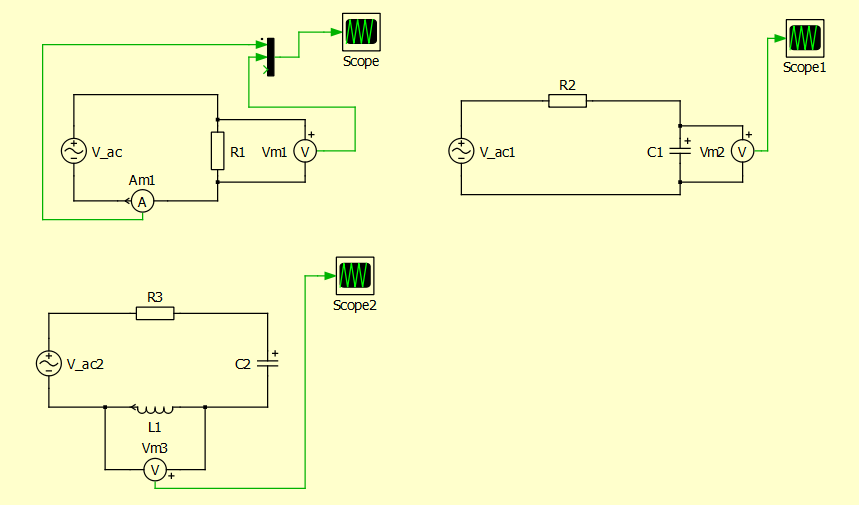
\includegraphics[width=1\textwidth]{Vildledning/Schematics/Eks1_LCR.png}
\caption{Foreslåede eksperiment kredsløb. R-kreds - CR-kreds - LCR-kreds}
\label{fig:Eks1}
\end{figure}
\newpage

\section{Hvad vil vi opstille?}
\begin{itemize}
\item R-kreds
\item CR-kreds
\item LCR-kreds
\end{itemize}
Til alle opstillingerne vil der i starten benyttes et oscilloskop som kilde, sat til vekselspænding ved 5 V, 50Hz.

De tre opsætninger benyttes som reference punkter til videre eksperimentring.  
\section{R-kreds}
Til at starte med vil vi opstille, det måske aller simpleste kredsløb, ved bare at sende en vekselspænding over en resistor og måle spændingsforskellen og strømmen over det.

Herefter vha. $U=R\cdot I$ kan der så undersøges om den aflæste værdi af resistoren er den samme som den målte.
\section{CR-kreds}
Opstillingen her er ens med R-kredsen, uden ampere-meter, bare at der nu er sat en kapacitator på og volt-meteret er flyttet hen over kapacitatoren.

Herefter ses der på om der er sket en ændring i spændingsforskellen over kapacitatoren, sammenlignet med den mængde spænding der er tilført systemet.
\section{LCR-kreds}
Dette er den vigtigste kreds der undersøges, da der nu er lavet et loop ved at sætte en spole i kredsløbet. Volt-meteret der benyttes her skulle gerne være et der kan tegne grafer, specifikt $(U,t)$.

Kredsløbet er en forlængelse af de to andre. Volt-meteret er nu bare flyttet til hen over spolen, da dette er den komponent med størst relevans.

Her undersøges der den spændingskurve der kan tegnes over spolen. Denne kan herefter sammenlignes med kurven i givet fra en simulering i Plecs. Dette er selvfølgelig kun relevant hvis det er muligt at komme tæt på virkelige værdier i programmet.

	\end{folderinput}

\bibliography{bib/bibfil} %% Litteraturlisten indsættes her %%

%\chapter{PV-fremadrettet}
Nu da vi har lavet vores første forsøg, hvor vi har set på, hvordan spændingen skifter over en modstand, kapacitator og spole ved ændring på frekvensen, kan vi nu gå videre til vores forsøg om WPT. Vi fik chancen for at omlægge den teori, vi har læst om, ud til en forsøgsopstilling, hvor vi kunne aflæse forskellige resultater, der giver mulighed for videre arbejde. Det har ikke lokket os fra at skulle arbejde videre med projektet, snarere det modsatte. Vi har fået nyt blod på tanden og glæder os til de afsluttende forsøg. Forsøgene skal benyttes til databehandlingen, så vi kan sammenligne resultaterne, så vi har konkrete tal at arbejde ud fra, når vi skal videre med problemløsningen. Vores strategi for fremtiden er at vi vil skriftes til at lave forsøg og dobbelttjekke hinandens forsøgsopstillinger. Når den ene del af gruppen er i laboratorierne vil den anden del af gruppen ihærdigt skriver videre, laver beregninger, skematics osv. til rapporten. Det er vores målsætning at holde møde hver fredag, så vi kan holde trit med vores tidsplan, og at hvis vi kommer bag ud, er det muligt for de andre i gruppen at træde til og hjælpe et medlem. Dette er ingen individuel rapport, og vi skal alle sammen kunne stå inde for rapporten. Ergo er det vigtigt, at man hjælper hinanden, for hvis der er en som taber, taber hele gruppen. Det er lige meget hvis skyld, det er, for vi er alle i samme båd.

For at holde gejsten oppe i gruppen sørger vi for at holde hinanden i nakken, så der ikke er nogen, der får problemer og falder bagud i forhold til gruppen. Projektet er en samlet indsats, så det er vigtigt at få lavet opsamlinger i gruppen, så alle kan følge med, og alle har samme udgangspunkt for senere arbejde. Derudover diskuterer vi om, hvad der interesserer os ved projektet, og hvad vi gerne vil have ud af det færdige produkt, så det holder os fast på et endeligt mål. Hvis vi arbejder med det, vi finder interesse for, er det lettere at holde sig fokuseret på arbejdsopgaverne, og man får lyst til at gøre en god indsats (ikke kun for en selv, men også for gruppen som helhed).

Som gruppe bliver vi enige om, hvilke arbejdsområder vi skal undersøge og skrive om. Herefter inddeler vi os i mindre grupper for hver arbejdsopgave (2-3 mand pr. gruppe). Dette gør, at vi hurtigt kan få indsamlet brugbar viden og udført en stort stykke arbejde, men at vi samtidig ikke står alene med en opgave. Det at være i små grupper gør også, at man kan få flere input og idéer til, hvad man eventuelt kan bringe ind over opgaven, hvilket gør at projektet bliver mere nuanceret. For at holde styr på, hvor langt hver gruppe er, og hvad de hver især har skrevet, så holder vi jævnligt møder til at opsummere processen.

Da vi er igennem problemanalysen, så har vi fået dannet os en god grundviden om projektet, som vi videre kan benytte til forsøg, modeller og projektløsningen senere hen. Dette betyder også, at vi nu skal til at specificere os på enkelte dele af projektet, så vi får indsnævret vores undersøgelser.

\end{document}